\chapter{Preliminaries and Related Work}\label{preliminaries}

In this chapter, we present the preliminaries and related works on natural bird's flocking model, multi-UAV formations and quadrotor model.

\section{Flocking}\label{flocking}

\subsection{Neighbors within Radius $r$}

Based on observations and previous work~\cite{Reynolds1987}, a model with novel type of dynamics (\ref{eq:vicsek}) has been proposed by Vicsek in~\cite{Vicsek1995} and the relationship between the coherence of flocking and the density of particles has been discussed. Each particle has constant velocity, while its direction is determined by ${\langle\theta(t)\rangle}_r$, which is the average direction of the neighboring particles within radius $r$ and $\Delta\theta$ represents the noise.
\begin{equation}\label{eq:vicsek}
\begin{aligned}
x_i(t+1)&=x_i(t)+v_i(t)\Delta t\\
\theta(t+1)&={\langle\theta(t)\rangle}_r+\Delta\theta
\end{aligned}
\end{equation}
where $x_i(t)$ represents the position of agent $i$ at time $t$, $v_i(t)$ represents the velocity of agent $i$ at time $t$ and $u_i(t)$ represents the input of agent $i$ at time $t$ (\ref{eq:motion}). The weight function $a_{ij}:\mathbb{E}^k\to[0,\infty)$ (\ref{eq:motion}) qualifies the influence of agent $j$ on agent $i$, which is a function of agents' positions. The detailed expression of $a_{ij}$ could be found at (\ref{eq:vicsek_aij}, \ref{eq:cs_aij}). The various properties of the flocking depend on the choices of different $a_{ij}$.

Considering a flock of $k$ agents labeled by $i=1,...,k$, moving in the $N$-dimensional Euclidean space. The motion of each agent in continuous time is described by double integrators as:
\begin{equation}\label{eq:motion}
\begin{aligned}
\dot{x_i}(t)&=v_i(t)\\
\dot{v_i}(t)&=u_i(t)\\
u_i(t)&=\underbrace{\sum^k_{j=1}a_{ij}(x)(v_j(t)-v_i(t))}_{\text{velocity-consensus term}}-\underbrace{\bigtriangledown_{x_i}V_i}_{\text{gradient-based term}}
\end{aligned}
\end{equation}
In above Vicsek's model, $a_{ij}$ is equally defined as (\ref{eq:vicsek_aij}), an example of $a_{ij}$ is shown in Figure~\ref{fig:v_aij}.
\begin{equation}\label{eq:vicsek_aij}
a_{ij}(x)=\left\{\begin{array}{rcl}
1, & & {if\ ||x_i-x_j||\leq R}\\
0, & & {otherwise}
\end{array} \right.
\end{equation}

\begin{figure}[htb]
  \centering
  \subfigure[$a_{ij}(x)$ with $R=1$ in~\cite{Vicsek1995}]{\label{fig:v_aij}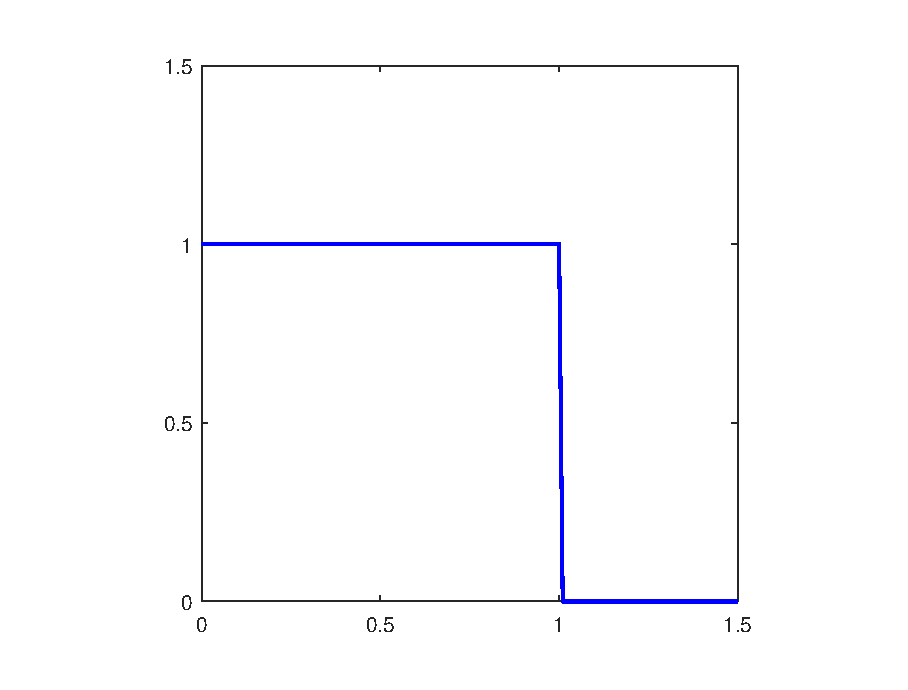
\includegraphics[width=0.48\textwidth]{figure/vicsek_aij.eps}}
  \subfigure[$a_{ij}(x)$ with $\sigma=1$, $K=1$ and $\beta=0.48$ in~\cite{CuckerSmale2007}]{\label{fig:cs_aij}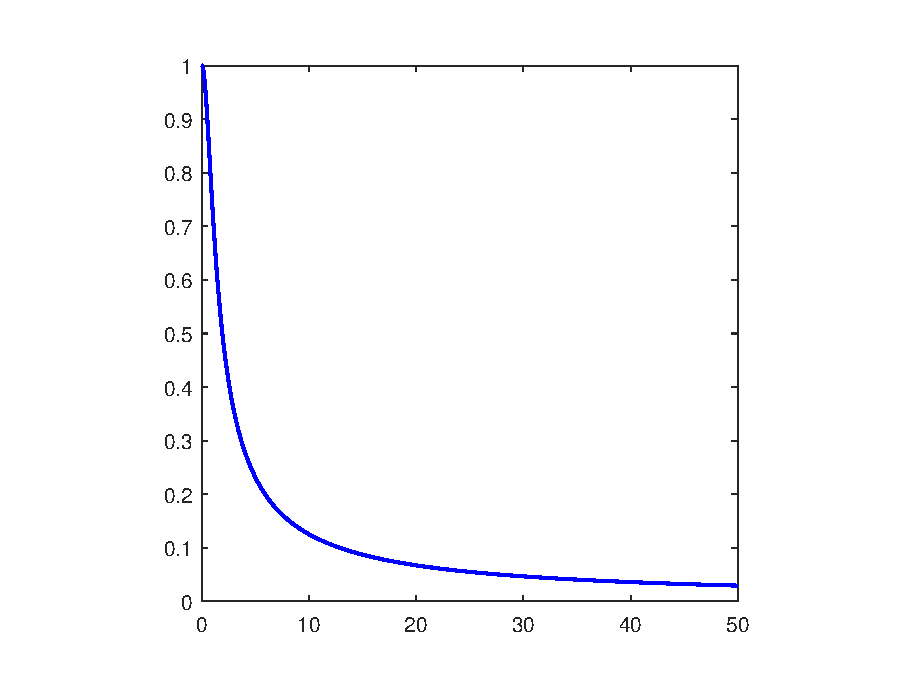
\includegraphics[width=0.48\textwidth]{figure/cs_aij.eps}}
  \caption{Examples of $a_{ij}(s)$ in~\cite{Vicsek1995},~\cite{CuckerSmale2007}}\label{fig:example_v}
\end{figure}

In natural flocking, however, the velocity of each bird is various that Vicsek's model can not be simply applied. Nor the cohesion and collision avoidance can be guaranteed. Given $\beta<\frac{1}{2}$ and proposed $a_{ij}$ (\ref{eq:cs_aij}, Figure~\ref{fig:cs_aij}),~\cite{CuckerSmale2007} has proved the convergence of the flock to a common velocity for both continuous and discrete time.
\begin{equation}\label{eq:cs_aij}
a_{ij}(x)=\frac{K}{(\sigma^2+||x_i-x_j||^2)^{\beta}}
\end{equation}
Based on this,~\cite{CuckerDong2010} has further proved the cohesion and separation of the flocks with condition $\beta\leq\frac{1}{2}$, by modifying the updating rule of $u_i(t)$ in (\ref{eq:motion}) to (\ref{eq:dong_aij}).
\begin{equation}\label{eq:dong_aij}
\begin{aligned}
u_i(t)&=\sum^k_{j=1}a_{ij}(x)(v_j(t)-v_i(t))+\Lambda(v)\underbrace{\sum_{j\neq i}f(||v_i-v_j||^2)(x_i-x_j)}_{\text{collision-avoidance term}}\\
\Lambda(v)&=(\frac{1}{k}\sum_{i>j}||v_i-v_j||^2)^{\frac{1}{2}}
\end{aligned}
\end{equation}
where $f:(d_0,\infty)\to[0,\infty)$ is any repelling function satisfies: for any $d>d_0$,
\begin{equation}\label{eq:dong_f}
\begin{aligned}
\int_{d_0}^d f(r)dr&=\infty\\
\int_d^{\infty} f(r)dr&<\infty
\end{aligned}
\end{equation}
An example $f(r)$ is illustrated in Figure~\ref{fig:dong_f}.
\begin{figure}[htb]
  \centering
  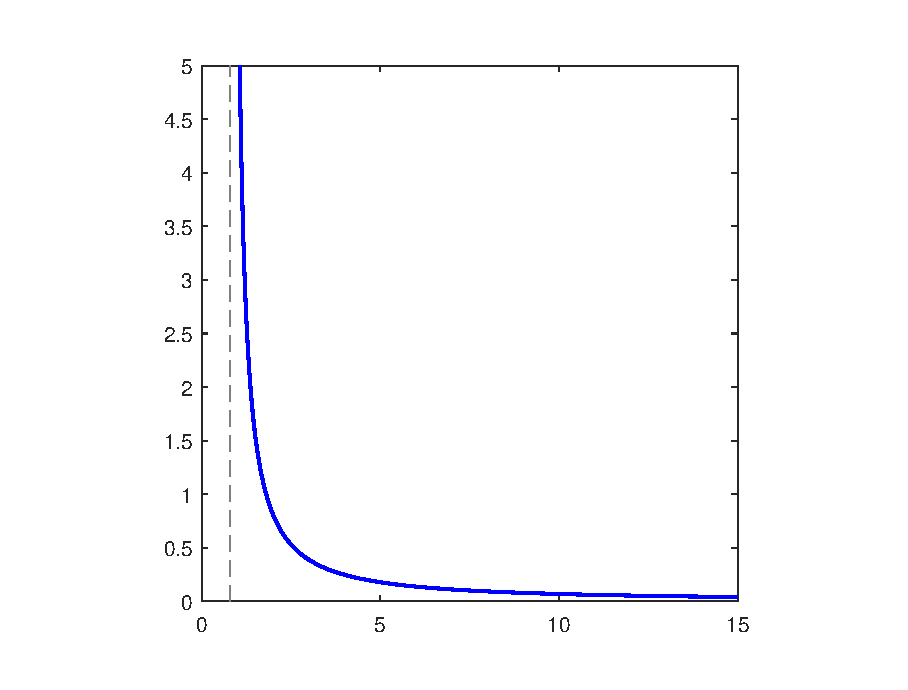
\includegraphics[width=0.48\textwidth]{figure/dong_f.eps}
  \caption{$f(r)$ with $d_0=0.8$ and $\theta=1.2$ in ~\cite{CuckerDong2010}}
  \label{fig:dong_f}
\end{figure}

\subsection{$K$ Nearest Neighbors}

Unlike above mentioned theories assume, \cite{PNAS} discovered that interaction between agents in flocking does not depend on the metric distance but rather on the topological distance. An average number of six to seven neighbors are involved in the interaction instead of neighbors within a fixed distance. An example is illustrated in Figure~\ref{fig:knn}, when $q=3$, three closest neighbors of agent 1 and agent 5 are agents 2, 3 and 6 and agents 1, 4 and 6 respectively. Given conditioned initial starting position, velocity and modified $a_{ij}$ (\ref{eq:martin_aij}),~\cite{Martin2014} has proved the alignment of the velocity in flocks.
\begin{equation}\label{eq:martin_aij}
a_{ij}(x)=\left\{\begin{array}{rcl}
1, & & {if\ j\in q\   closest\    neighbors\  of\ i}\\
0, & & {otherwise}
\end{array} \right.
\end{equation}

\begin{figure}[htb]
  \centering
  \includegraphics[width=0.5\textwidth]{figure/knn.eps}
  \caption{A flock of six agents with $q=3$}
  \label{fig:knn}
\end{figure}

\noindent
Based on this,~\cite{CuckerDong2016} has further introduced the quotient $\frac{q}{k-1}$ that unconditional flocking occurs when $\frac{q}{k-1}\geq\frac{1}{2}$.

\section{Multi-UAV Formations}

There are four main methods for UAV formation at present, leader-wingman~\cite{Wingman}, artificial potential field (APF)~\cite{Martin2014,Martin2014,Saber2006}, virtual structure~\cite{Virtual2008,Askari2015} and behavior-based method~\cite{Zhang2018,Behavior2004,Reynolds1987,Vicsek2018,Martin2017,Cai2012} as shown in Figure~\ref{fig:multi_uav}. \textcolor{red}{TODO: Review more papers}
\begin{figure}[htb]
  \centering
  \subfigure[Leader-Wingman]{\label{fig:wingman}\includegraphics[width=0.48\textwidth]{figure/wingman.eps}}
  \subfigure[Artificial Potential Field]{\label{fig:apf}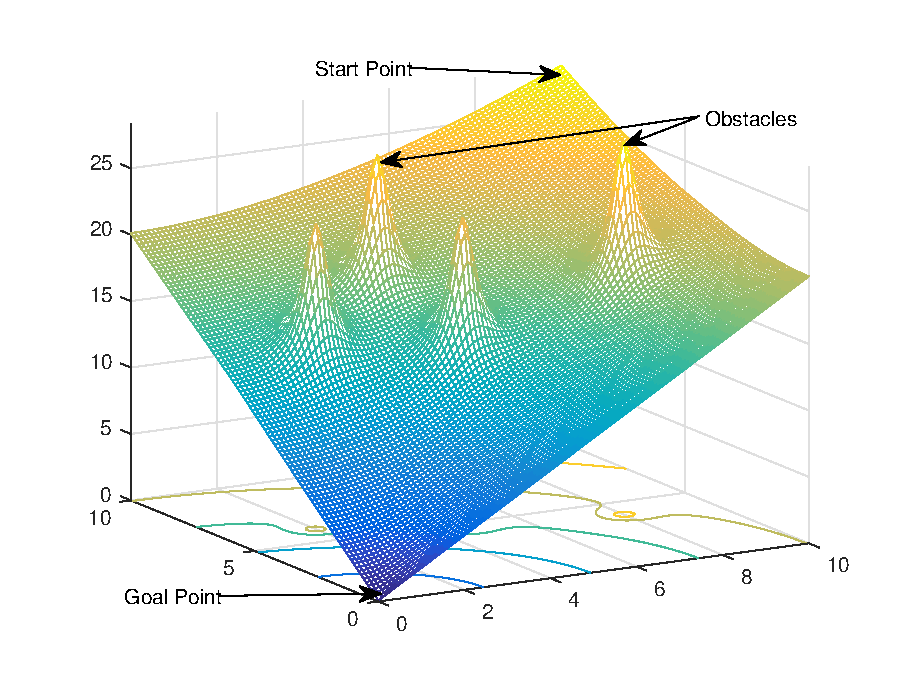
\includegraphics[width=0.48\textwidth]{figure/apf.eps}}
  \subfigure[Virtual Structure,~\cite{Askari2015}]{\label{fig:virtual}\includegraphics[width=0.48\textwidth]{figure/virtual.eps}}
  \subfigure[Behavior Based,~\cite{Cai2012}]{\label{fig:behavior}\includegraphics[width=0.48\textwidth]{figure/original/chapter_2/behavior.png}}
  \caption{Multi-UAV Formations}\label{fig:multi_uav}
\end{figure}

\subsection{Leader-Wingman}
The leader-wingman strategy originates from aerial combat, where leader aircraft takes the main role of missions with wingman flying beside or slightly behind, permitting the attack of enemies from back. In multi-UAV formation, wingman is required to keep a desired relative position and orientation from leader and maintain the formation, using information collected from leader-wingman communication, ground central computer or on-board perception system. In~\cite{Wingman} a communication free leader-follower formation is proposed, where only visual sensors are equipped on follower to obtain the relative poses from leader. The distribution of computation load from central computer to individuals enables a wider range of applications and reduces human operations, however, individuals are more vulnerable to sensor disturbance, especially in large scale formations.

\subsection{Artificial Potential Field}
Artificial potential field consists of repulsive and attractive potential fields. The goal position produces an attractive force, making the robot move towards it, while obstacles, neighbors and predators generates a repulsive force, pushing robots away from them. The total force applied to a robot in APF is the sum of both attractive and repulsive forces exerted at that position (An example is given in~\ref{eq:apf}, Figure~\ref{fig:apf}). The motion of a robot is then determined in the above field of forces and from positions with high potentials to low potentials. Inspired by~\cite{Reynolds1987},~\cite{Martin2014} proposed and integrated three potential functions for separation, alignment and cohesion movement of UAV flocks. Traditional APF method suffers from the problem of local minima, that the robot might be trapped at certain point where attractive and repulsive force are equal. Though modified potential functions and virtual agents have been proposed in~\cite{Saber2006}, parameter optimization is always a difficult task.
\begin{equation}\label{eq:apf}
\begin{aligned}
F_{att}&=\nabla U_{att}(x)=\nabla(\alpha||\mathbf{x}-\mathbf{x_g}||^2)=2\alpha(\mathbf{x_g}-\mathbf{x})\\
F_{rep}&=\nabla U_{rep}(x)=\nabla(\frac{1}{||\mathbf{x}-\mathbf{x_o}||^2+\beta})=\frac{2(\mathbf{x}-\mathbf{x_o})}{(||\mathbf{x}-\mathbf{x_o}||^2+\beta)^2}
\end{aligned}
\end{equation}

\subsection{Virtual Structure}
Virtual structure method embeds multi-UAVs into a virtual structure and treats it as a virtual single rigid body~\cite{Virtual2008}. A virtual leader is assigned at the virtual geometric center as a reference that each agent's desired pose could be defined relative to that leader, as shown in Figure~\ref{fig:virtual}. As a result, single UAV path planning and trajectory generation techniques can be employed for the virtual leader while trajectory tracking strategies can be employed for each UAV~\cite{Askari2015}. The stability of the virtual structure method strictly depends on each agent's knowledge of the virtual leader coordinate frame. When each agent has inconsistent understanding of the relative pose from virtual leader, the desired formation geometry could not be maintained. Moreover, altering formation shape is inflexible when facing dynamically changing environment.

\subsection{Behavior Based}
In behavior-based approach, control functions are separated into variety of function items and the whole function is then formed as the combination of different items. In multi-UAV formation, control function items are divided into three categories, task-related planning (search for goals), emergency proof operations (avoid obstacles) and information exchange (communicate with neighbors)~\cite{Behavior2004} as illustrated in Figure~\ref{fig:behavior}. In~\cite{Reynolds1987}, three behaviors are defined including collision avoidance with neighbors, local velocity alignment and global goal constraint. Each of these items are computed separately and then combined for movement. Based on this, a self-propelled multi-UAV flocking in bounded area and a collective target tracking multi-UAV formations have been proposed in~\cite{Vicsek2018}, however, the shape of the flocking is hard to maintain.


\section{Quadrotor Model}

\subsection{Coordinate Frame}

\begin{figure}[htb]
  \centering
  \includegraphics[width=1.0\textwidth]{figure/coordinate.eps}
  \caption{Coordinate frames of world, quadrotor body and on-board camera}
  \label{fig:coordinate}
\end{figure}
Three coordinate frames are introduced including world, quadrotor body and its on-board camera as illustrated in Figure~\ref{fig:coordinate}. In Chapter~\ref{implementation}, target quadrotor is captured in camera frame whose position is denoted by $\mathbf{p_c}\in\mathbb{R}^3$. For the simplicity and unity of the calculations, $\mathbf{p_c}$ is transformed back to world frame $\mathbf{p_w}\in\mathbb{R}^3$ by $\tensor*[^w]{\mathfrak{g}}{_c}\in\mathbb{R}^{4\times4}$:
\begin{equation}\label{eq:transform}
\begin{aligned}
\begin{bmatrix}\mathbf{p^T_w}&1\end{bmatrix}^T&=\tensor*[^w]{\mathfrak{g}}{_c}\begin{bmatrix}\mathbf{p^T_c}&1\end{bmatrix}^T\\
\tensor*[^w]{\mathfrak{g}}{_c}&=\tensor*[^w]{\mathfrak{g}}{_b}\tensor*[^b]{\mathfrak{g}}{_c}=\begin{bmatrix}\mathbf{\tensor*[^w]{R}{_b}}&\mathbf{\tensor*[^w]{p}{_b}}\\\mathbf{0^{1\times3}}&1\end{bmatrix}
\begin{bmatrix}\mathbf{\tensor*[^b]{R}{_c}}&\mathbf{\tensor*[^b]{p}{_c}}\\\mathbf{0^{1\times3}}&1\end{bmatrix}\\
\tensor*[^b]{\mathbf{R}}{_c}&=\mathbf{R_z}(\psi)\mathbf{R_y}(\theta)\mathbf{R_x}(\phi)
\end{aligned}
\end{equation}
where $\mathbf{p_c}$ is first rotated w.r.t $z_c$ by yaw angle $\psi$, then $z_y$ by pitch angle $\theta$, last $z_x$ by roll angle $\phi$ and shifted by $\tensor*[^b]{\mathbf{p}}{_c}$ to $\mathbf{p_b}$ in body frame. Iteratively, $\mathbf{p_c}$ is transformed back to $\mathbf{p_W}$ in world frame (\ref{eq:transform}). It is worthwhile to point out that both $\tensor*[^b]{\mathfrak{g}}{_c}$ and $\tensor*[^w]{\mathfrak{g}}{_b}$ are estimated online by ~\cite{VINS} in Chapter~\ref{hardware}. The $\mathbf{R_z}(\psi)$, $\mathbf{R_y}(\theta)$ and $\mathbf{R_x}(\phi)\in\mathfrak{SE(3)}$ are rotation matrixes.
\begin{equation}\label{eq:rotation}
\begin{aligned}
R_z(\psi)&=\begin{bmatrix}cos\psi&-sin\psi&0\\sin\psi&cos\psi&0\\0&0&1\end{bmatrix}\\
R_y(\theta)&=\begin{bmatrix}cos\theta&0&sin]\theta\\0&1&0\\-sin\theta&0&cos\theta\end{bmatrix}\\
R_x(\phi)&=\begin{bmatrix}1&0&0\\0&cos\phi&-sin]\phi\\0&sin\phi&cos\phi\end{bmatrix}
\end{aligned}
\end{equation}

\subsection{Quadrotor Dynamics and Kinematics}

The center of mass of quadrotor body in world frame is denoted by $\mathbf{r}\in\mathbb{R}^3$, then from Newton's law we have:
\begin{equation}\label{eq:newton}
m\mathbf{\ddot{r}}=\begin{bmatrix}0\\0\\-mg\end{bmatrix}+\tensor*[^w]{\mathbf{R}}{_b}\begin{bmatrix}0\\0\\\sum F_i\end{bmatrix}
\end{equation}
where $\mathit{m}\in\mathbb{R}$ is the total weight of the quadrotor and $\mathit{F_i}\in\mathbb{R}$ is the lifting force provided by each motor. The components of the angular velocities of quadrotor in its body frame are denoted by $\mathit{p}$, $\mathit{q}$ and $\mathit{r}\in\mathbb{R}$ and are related with $\theta$, $\phi$ and $\psi\in\mathbb{R}$ by:
\begin{equation}\label{eq:pqr}
\begin{bmatrix}p\\q\\r\end{bmatrix}=\begin{bmatrix}cos\theta&0&-cos\phi sin\theta\\0&1&sin\phi\\sin\theta&0&cos\phi cos\theta\end{bmatrix}\begin{bmatrix}\dot{\phi}\\\dot{\theta}\\\dot{\psi}\end{bmatrix}
\end{equation}

In addition to force, each motor has also produced moment, $\mathit{M_i}\in\mathbb{R}$, perpendicular to $x_b-x_y$ plane. We denote the length from each motor to the center of mass by $\mathit{L}\in\mathbb{R}$ and the moment of inertia matrix along $x_b-y_b-z_b$ axes by $\mathbf{I}\in\mathbb{R}^{3\times3}$. We then have the following Euler equations:\textcolor{red}{TODO: Modify Euler equations}
\begin{equation}\label{eq:euler}
\mathbf{I}\begin{bmatrix}\dot{p}\\\dot{q}\\\dot{r}\end{bmatrix}=\begin{bmatrix}L(F_2-F_4)\\L(F_3-F_1)\\M_1-M_2+M_3-M_4\end{bmatrix}-\begin{bmatrix}p\\q\\r\end{bmatrix}\times
\mathbf{I}\begin{bmatrix}p\\q\\r\end{bmatrix}
\end{equation}

\begin{figure}[htb]
  \centering
  \includegraphics[width=1.0\textwidth]{figure/original/chapter_2/nest.png}
  \caption{Nested control loops for position and attitude control,~\cite{GRASP}}
  \label{fig:nest}
\end{figure}

As shown in Figure~\ref{fig:nest}, the control loops are divided into inner attitude control and outer position control. With the help of DJI Onboard SDK and owing to the differential flatness property, the state and input could be represented as algebraic functions of four carefully selected flat outputs $[\mathbf{r}^T, \psi]$ and their derivatives~\cite{Snap}. This facilitates the generation of trajectories since any smooth trajectory (with reasonably bounded derivatives) in the space of flat outputs can be followed by the quadrotor. Thus the main work of quadrotor motion planning goes to the design of the required trajectory.


\newpage